%!TEX root = ../../thesis.tex

\section{Interaction frame hypothesis}
\label{chapter:limitations:framehypothesis}

\question{How to relax the assumption that interaction frame is pre-defined and unique?}

Until now we have assumed that the interaction frame, which specifies the details of the interaction between the human and the machine was known. In this section, we considered the case where multiple interaction frames are defined, but only one of them accounts for the interaction between the human and the machine.

% In this frame only the meaning of the signal was unknown. 

\subsection{Illustrations}

We will use a very simple example to illustrate the problem and show computational results. We consider that the agent lives in the line word as defined in chapter~\ref{chapter:lfui::symmetries}, where the agent has access to the ``no move'' action in order to remove the symmetry problem. The agent knowns it should reach either of the two edges of the world, G1 or G2. And the agent knowns that the teacher is providing either feedback or guidance instructions. To handle this new hidden information we will rely again on our interpretation hypothesis process. This time, one hypothesis will be the combination of one task hypothesis and one frame hypothesis. For our simple example, it results in having four hypotheses.

The result of the labeling process is shown in Figure~\ref{fig:multipleframeexplainedfeedback} for a teacher providing feedback instructions according the task G1. The hypothesis that labels the signals according to the task G1 and the feedback frame is the one whose signal-label pairs match better with the underlying structure of the data. Indeed, for the guidance case, the labeling process for hypothesis G1 is always giving a ``left'' label whether or not the agent is moving away or closer to the target, which allows to differentiate between feedback and guidance cases. To differentiate between G1 and G2, the same principle than the one described in chapter~\ref{chapter:lfui::symmetries} applies.

\begin{figure}[!htbp]
\centering
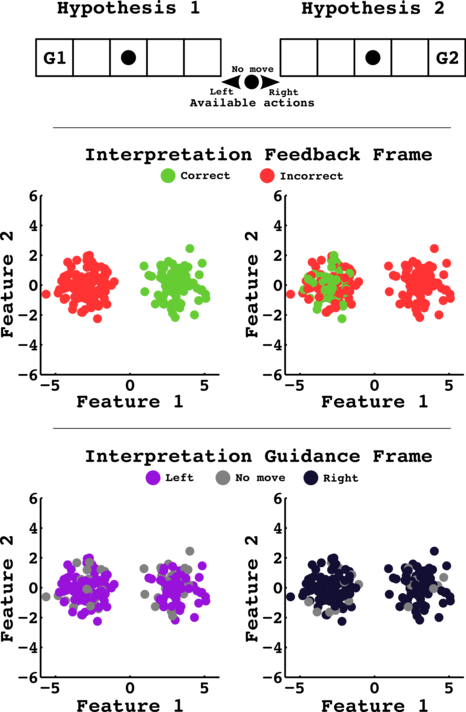
\includegraphics[width=\twoplanningwidth\columnwidth]{\visualspdf/multiple_frame/multiple_frame_feedback.pdf}
\caption{Illustration of the labeling process on both task and interaction frame hypothesis. The agent can perform right, left, or a ``no move'' action. The agent receive feedback on its action in the line word according to G1 . The agent do not known which task (G1 or G2) neither which interaction scheme the teacher is following (feedback or guidance). The result of the labeling process allow to identify the hypothesis on task G1 and feedback frame as the more likely.}
\label{fig:multipleframeexplainedfeedback}
\end{figure} 

Considering now that the teacher is providing guidance instructions according the task G1, the results of the labeling process can be seen in Figure~\ref{fig:multipleframeexplainedguidance}. The same explanation than for Figure~\ref{fig:multipleframeexplainedfeedback} applies. 

\begin{figure}[!htbp]
\centering
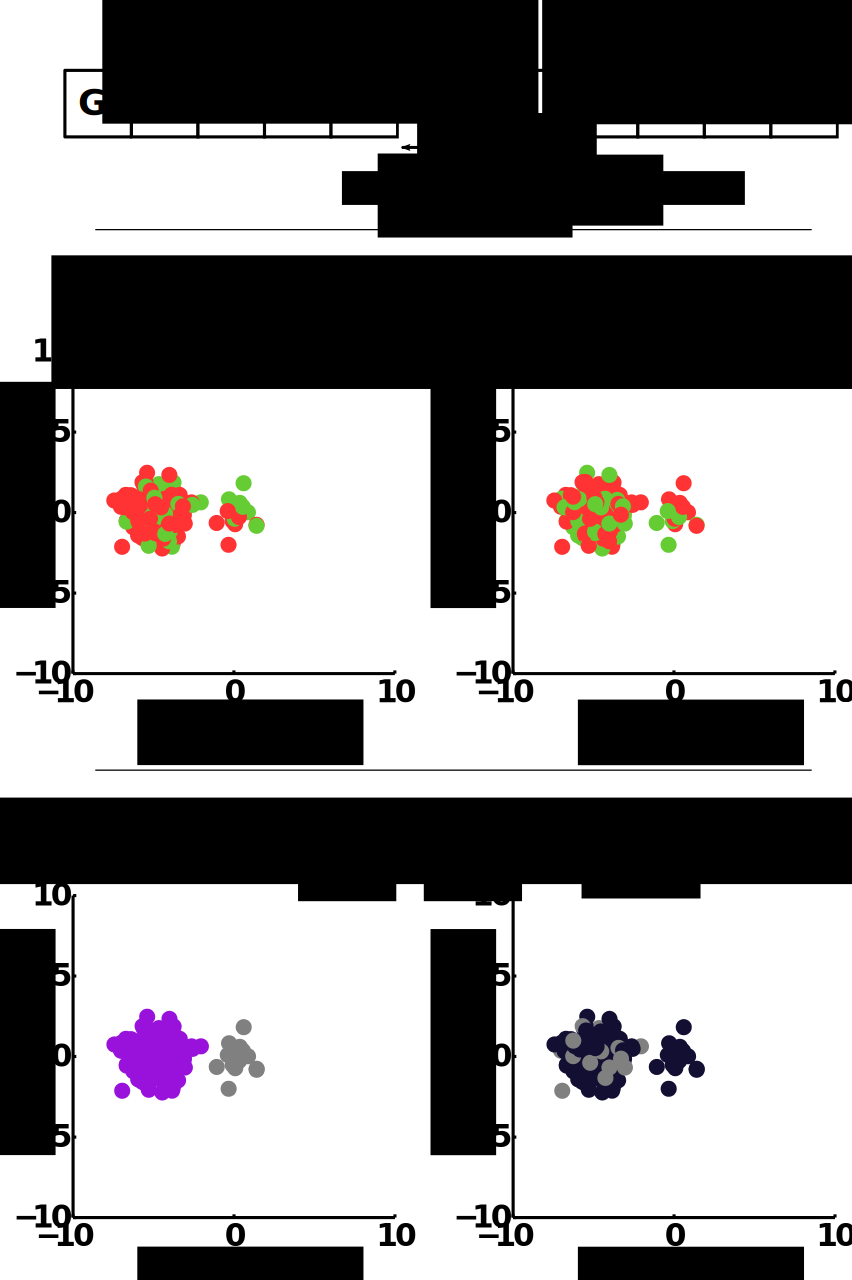
\includegraphics[width=\twoplanningwidth\columnwidth]{\visualspdf/multiple_frame/multiple_frame_guidance.pdf}
\caption{Illustration of the labelling porcess on both task and interaction frame hypothesis. The agent can perform right, left, or a ``no move'' action. The agent receive guidance instruction on its action in the line word according to G1 . The agent do not known which task (G1 or G2) neither which interaction scheme the teacher is following (feedback or guidance). The result of the labeling process allow to identify the hypothesis on task G1 and guidance frame as the more likely.}
\label{fig:multipleframeexplainedguidance}
\end{figure} 

\subsection{Simple experiments}

We now verify that the algorithm works in practice. We consider the same line world scenario as described above. For our experiments, the simulated teacher selects randomly a target (G1 or G2) and an interaction frame (feedback or guidance). The agent is using our uncertainty based planning method. We ran 100 simulations. All other settings were set as for the experiments of chapter~\ref{chapter:planning:method}.

Figure~\ref{fig:multipleframeall} shows the evolution of the probability associated to the correct combination of task and interaction frame (we use the minimum of pairwise normalized likelihood from Equation~\ref{eq:probapairwise} in chapter~\ref{chapter:lfui:confidence}). After 200 steps, all our experiments identified with probability 1 the correct combination of task and interaction frame. 

% In practice, in our previous experiments, we used a confidence threshold of 0.9, under this condition most of our experiments would have identified the task in slighlty more than 50 steps.

\begin{figure}[!htbp]
\centering
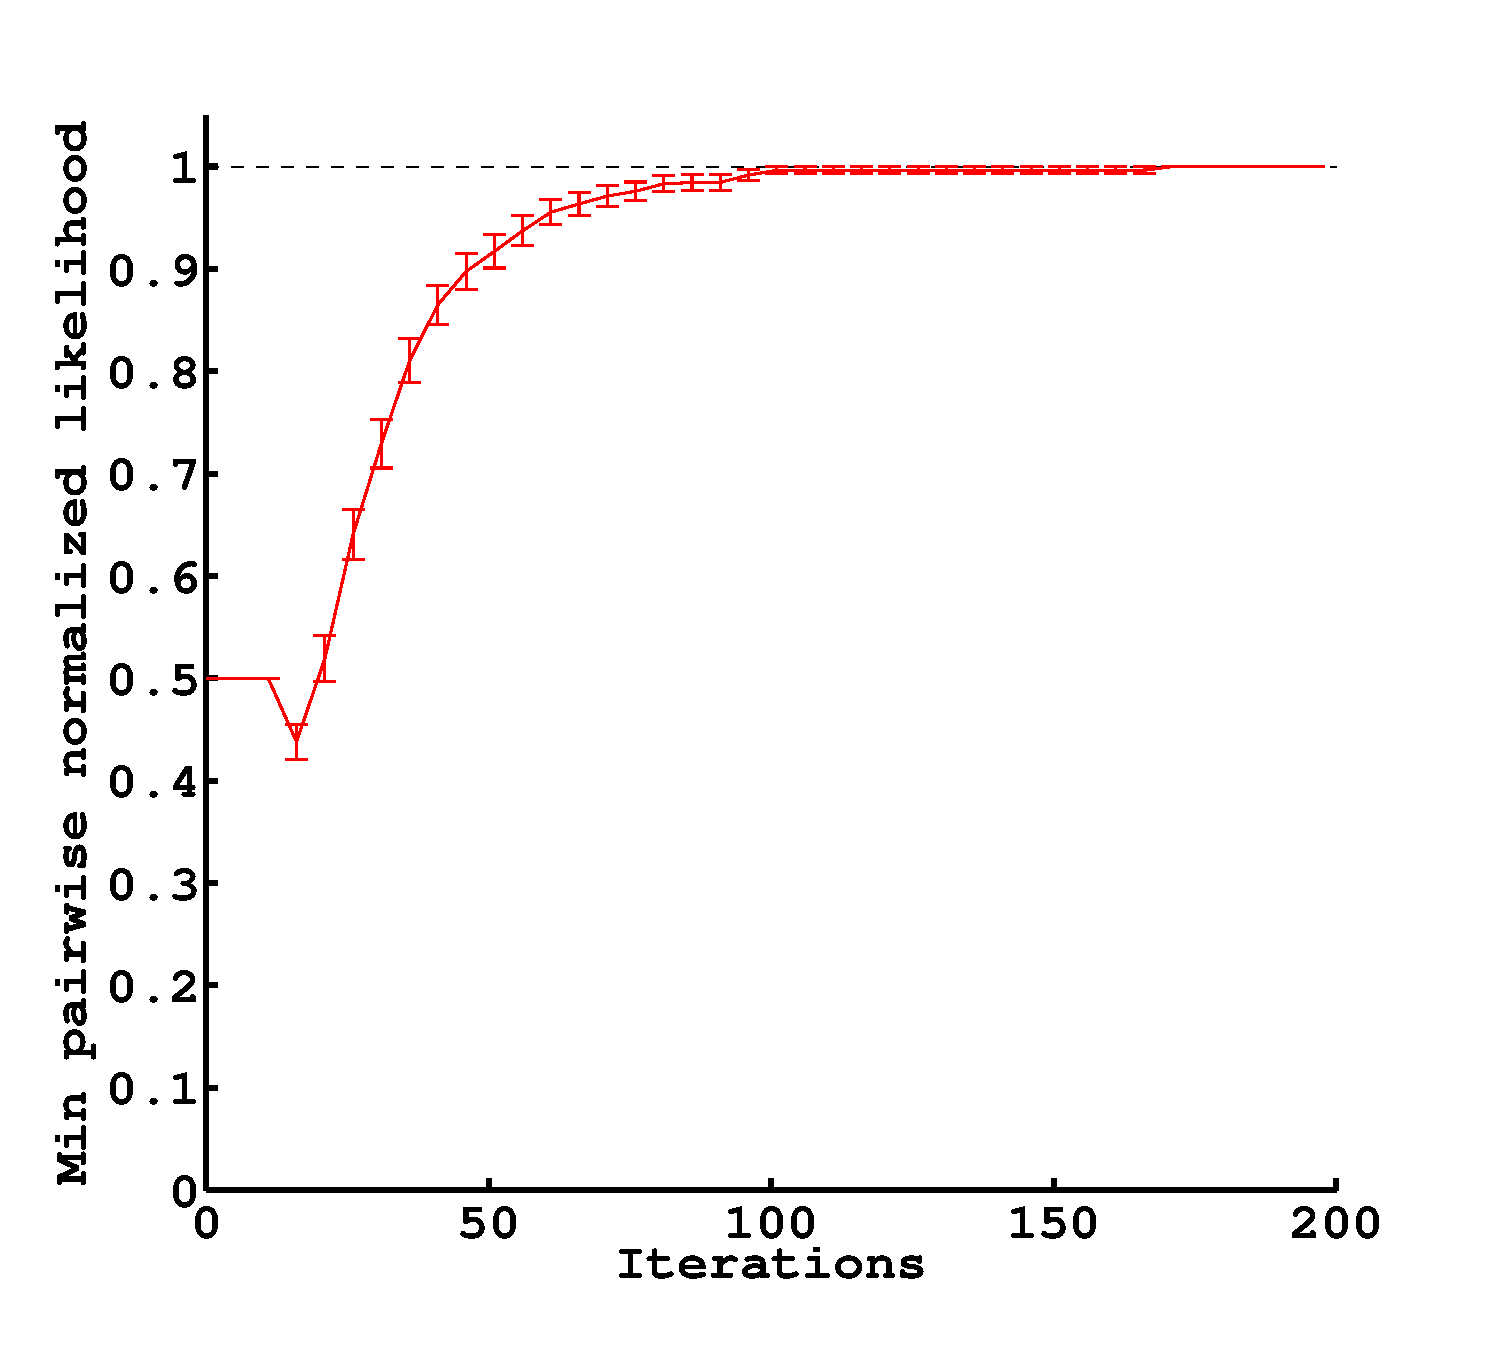
\includegraphics[width=\plotsize\columnwidth]{\imgpath/multiple_frame/multiple_frame_all_teacher.eps}
\caption{Evolution of the minimum of pairwise normalized likelihood for the correct hypothesis. After 200 steps, all our experiments identified with probability 1 the correct combination of task and interaction frame. Most of the experiments would have identified the task slighlty more than 50 steps with a confidence threshold of 0.9.}
\label{fig:multipleframeall}
\end{figure} 

We plot in Figure~\ref{fig:multipleframefeedbackvsguidance} the cases where the teacher was using the feedback frame (left) or the guidance frame (right). The performance are similar in both cases.

\begin{figure}[!htbp]
\centering
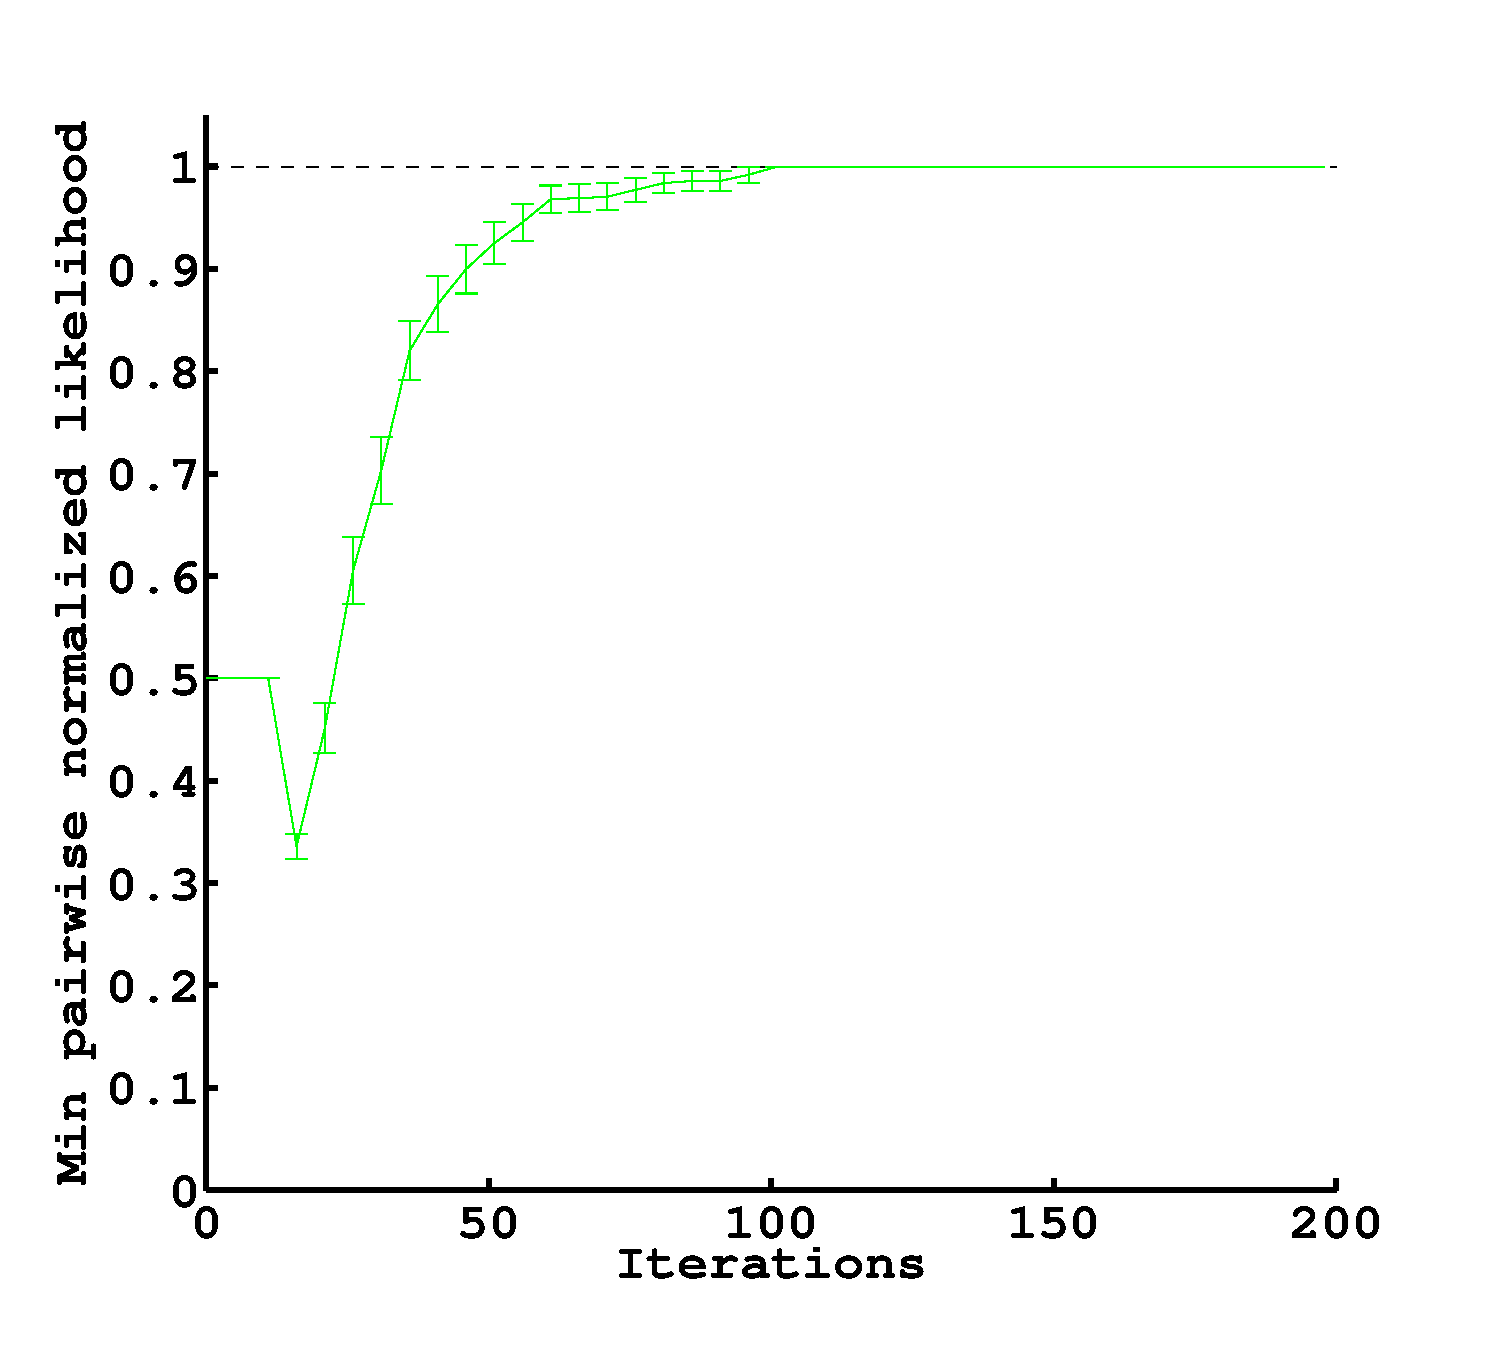
\includegraphics[width=0.49\columnwidth]{\imgpath/multiple_frame/multiple_frame_feedback_teacher.eps}
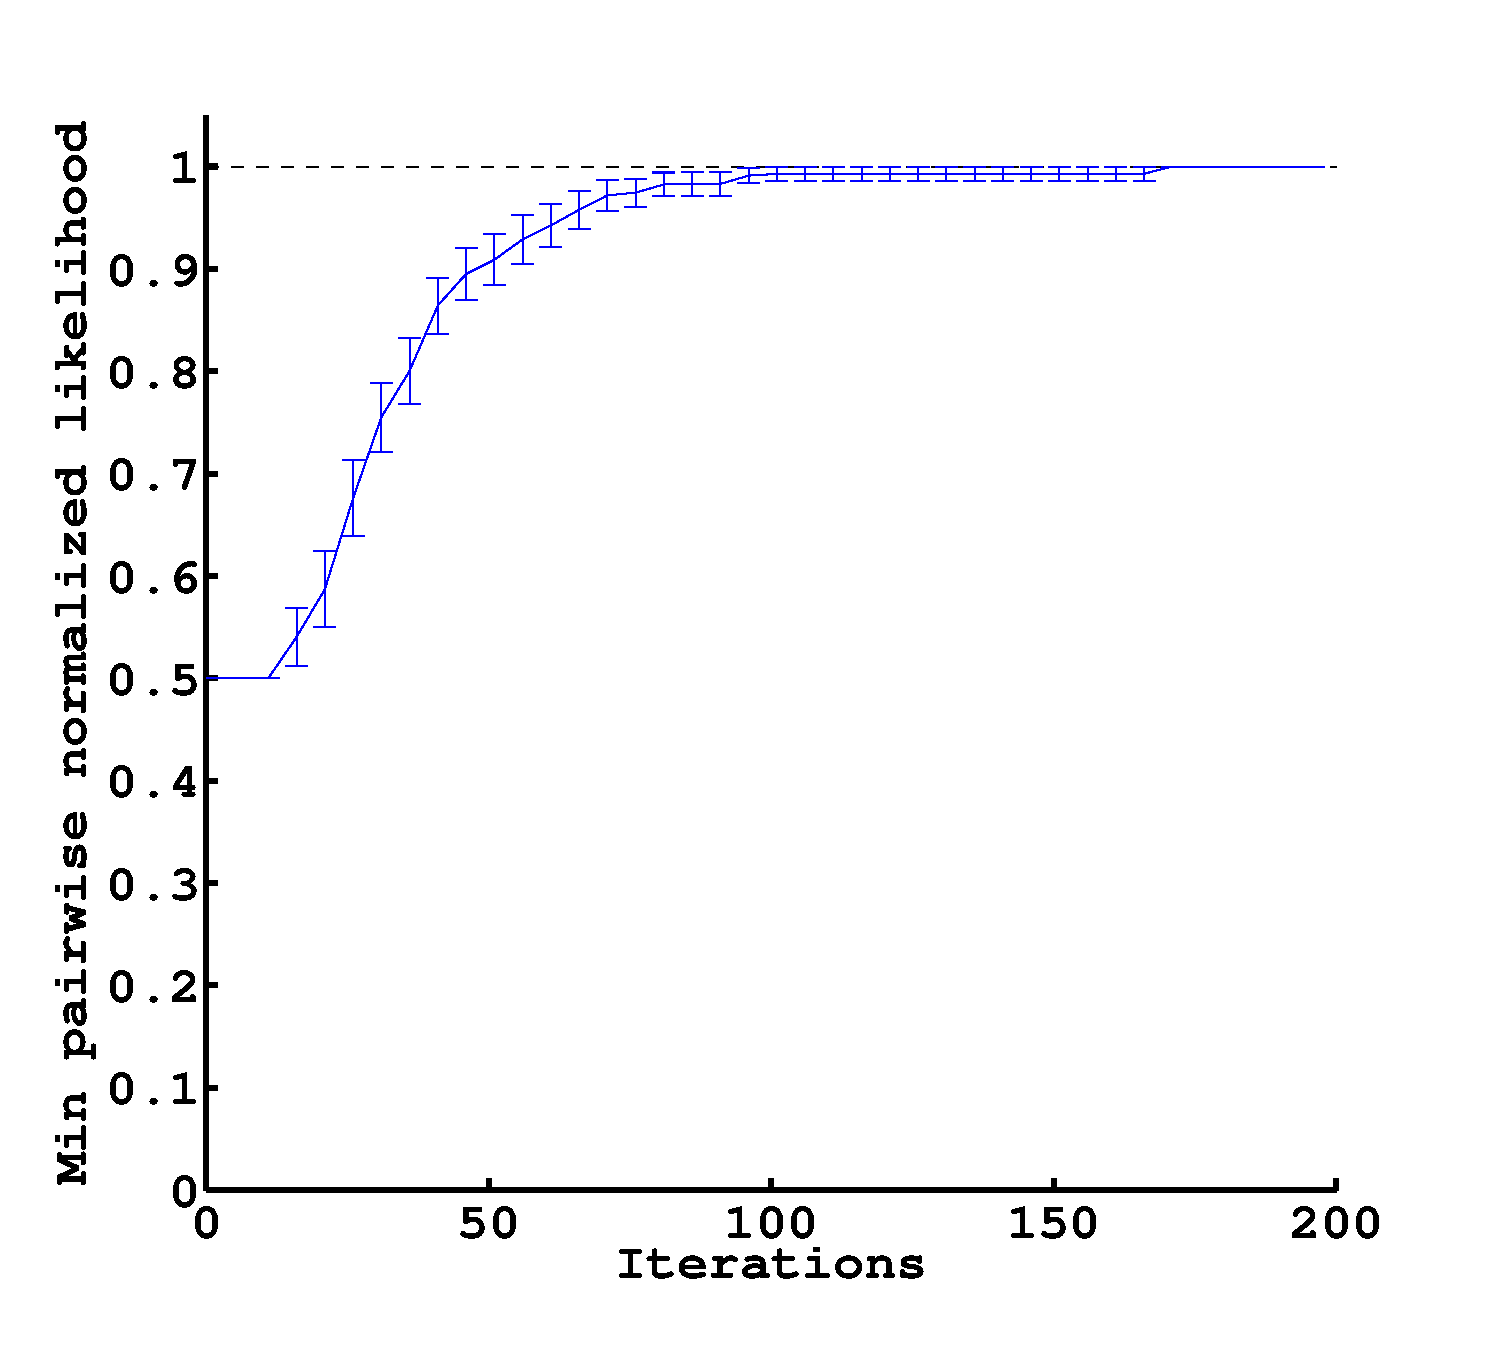
\includegraphics[width=0.49\columnwidth]{\imgpath/multiple_frame/multiple_frame_guidance_teacher.eps}
\caption{Evolution of the minimum of pairwise normalized likelihood for the correct hypothesis if the teacher provided feedback (left) or guidance (right) instruction. After 200 steps, all our experiments identified with probability 1 the correct combination of task and interaction frame. Most of the experiments would have identified the task in slightly more than 50 steps with a confidence threshold of 0.9.}
\label{fig:multipleframefeedbackvsguidance}
\end{figure} 


\subsection{Discussion}

Following the interpretation hypothesis method on a combination of task and interaction frame, we can start learning a task from unlabeled instructions and undefined interaction frames. In other words, such system can not only learn the task and the signal to meaning mapping, but also the interaction protocol used by the teacher.

Considering our example in section~\ref{chapter:limitation:continuoushypothesis}, an application this method can be to consider different coordinate system for the cardinal frame. For example, the signals from the teacher can be relative to the true North magnetic pole, to the current position of the user relative to the agent, or relative to the current orientation of the robot. This experiment performed with a real robot, real users, considering a tablet, and different interaction frames has great potential to demonstrate the potential application of this work.

Finally, we note that a particle filter based method (as used in section~\ref{chapter:limitations:continoushypothesis} for dealing with continuous task) could be considered for dealing with a continuous set of interaction frames. For example, in our example of section~\ref{chapter:limitations:continousstate}, we used a parameterized frame that merged feedback and guidance frame (see Equation~\ref{eq:mixedfeedbackguidance}), and introduced a feedback to guidance ratio $\alpha$. By generating, testing, and resampling a set of $\alpha$, i.e. a set of interaction frames, we may be able to learn, not only the task and the signal to meaning mapping, but also the details of the interaction protocol used by the teacher.

 % For example, in the experiment of section~\ref{chapter:limitations:continousstate} we may identify automatically the $\beta$ parameter of Equation~\ref{eq:mixedfeedbackguidance}.